\documentclass[crop,tikz]{standalone}
\usepackage{physics}
\usetikzlibrary{positioning}

\begin{document}
% \tikzset{
%   font={\fontsize{12pt}{12}\selectfont}}
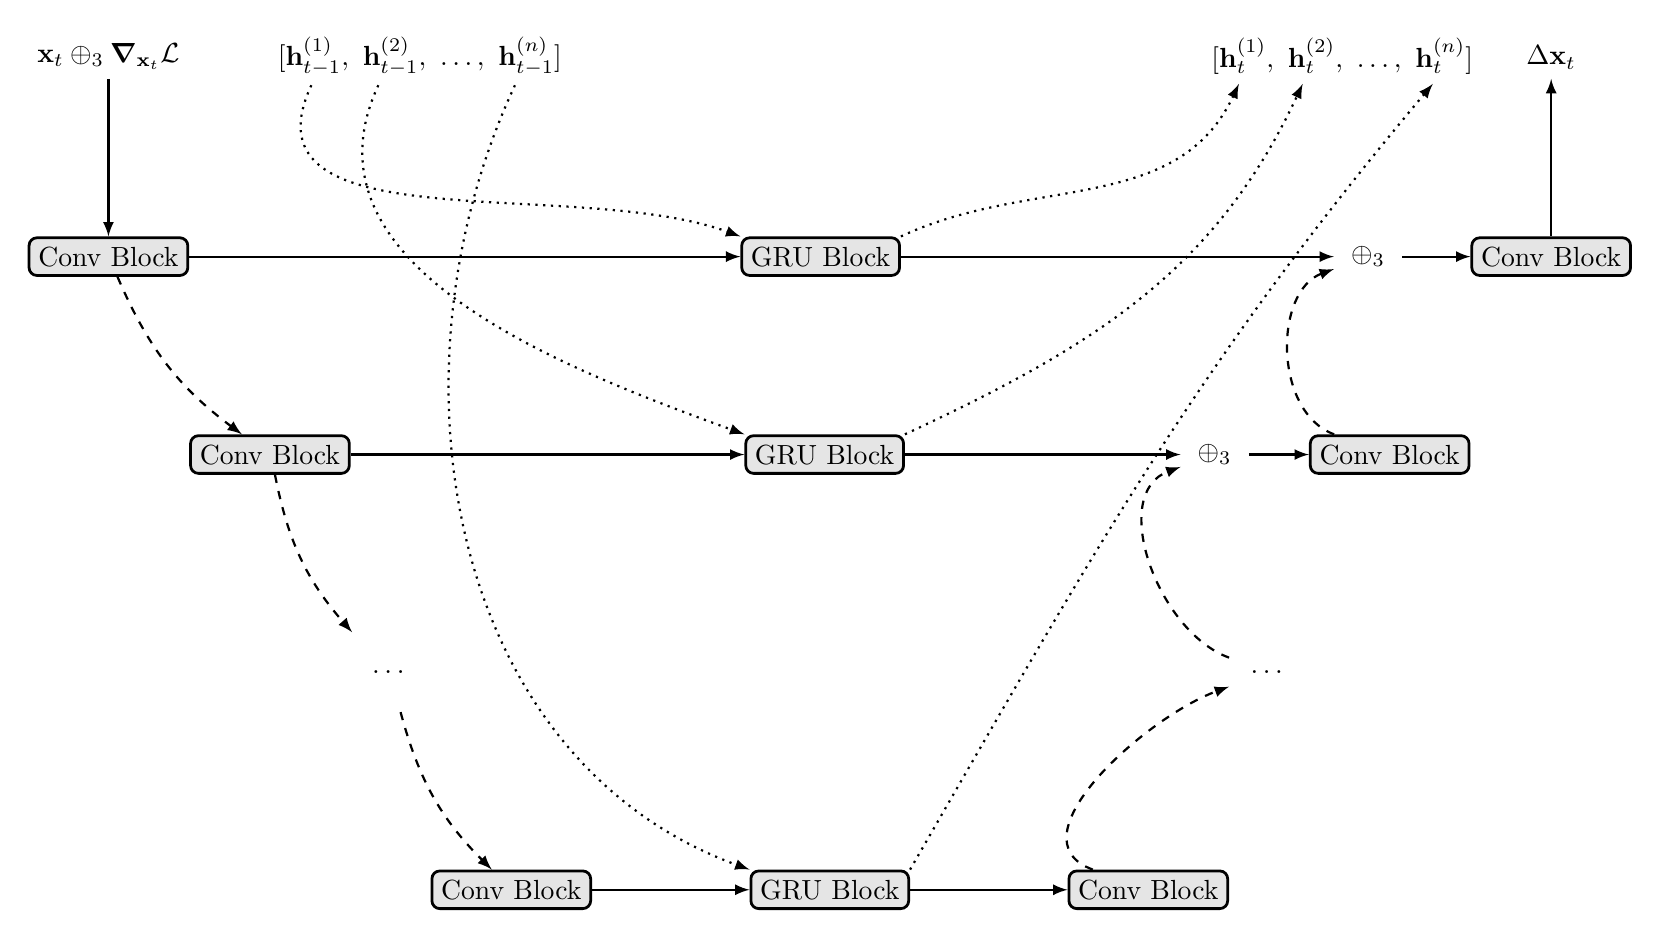
\begin{tikzpicture}[
  conv_node/.style={shape=rectangle, rounded corners=.1cm, draw=black, line width=1, fill=black!10},
  gru_node/.style={shape=rectangle, rounded corners=.1cm, draw=black, line width=1, fill=black!10},
  straight_edge/.style={-latex, thick},
  state_edge/.style={-latex, thick, dotted, out=245, in=160},
  state_edge_up/.style={-latex, thick, dotted, in=245, out=25},
  down_edge/.style={-latex, dashed, thick, bend right=15},
  up_edge/.style={-latex, dashed, thick, in=200, out=160},
  concat/.style={inner sep=6pt},
  node distance=3cm
]
    \node (input) at (0, 0) {$\mathbf{x}_t \oplus_3 \grad_{\mathbf{x}_t} \mathcal{L}$};
    \node (states) [right=1cm of input] 
    {$[\mathbf{h}^{(1)}_{t-1},\,\,
    \mathbf{h}^{(2)}_{t-1},\,\,
    \dots,\,\,
    \mathbf{h}^{(n)}_{t-1}]$};
    \node (output_states) [right=8cm of states] 
    {$[\mathbf{h}^{(1)}_{t},\,\,
    \mathbf{h}^{(2)}_{t},\,\,
    \dots,\,\,
    \mathbf{h}^{(n)}_{t}]$};
    
    % conv 1
    \node[conv_node] (conv1) [below=2cm of input] {Conv Block};
    \draw[straight_edge] (input) to (conv1);
    
    % conv 2
    \node[conv_node] (conv2) [below right=2cm and 0cm of conv1] {Conv Block};
    \draw[down_edge] (conv1) to (conv2);
    
    % Skip connection 1
    % \node[concat] (concat1_1) [right=3.5cm of conv1] {$\oplus_3$};
    % \draw[straight_edge] (conv1) to (concat1_1);
    % \draw[state_edge] (states.195) to (concat1_1);
    % \node[gru_node] (gru1) [right=3.5cm of concat1_1] {GRU Block};
    % \draw[straight_edge] (concat1_1) to (gru1);
    \node[gru_node] (gru1) [right=7cm of conv1] {GRU Block};
    \draw[straight_edge] (conv1) to (gru1);
    \draw[state_edge] (states.195) to (gru1.north west);
    \draw[state_edge_up] (gru1.north east) to (output_states.195);
    \node[concat] (concat1_2) [right=5.5cm of gru1] {$\oplus_3$};
    \draw[straight_edge] (gru1) to (concat1_2);
    
    
    % Skip connection 2
    % \node[concat] (concat2_1) [right=2.5cm of conv2] {$\oplus_3$};
    % \draw[straight_edge] (conv2) to (concat2_1);
    % \draw[state_edge] (states.215) to (concat2_1);
    % \node[gru_node] (gru2) [right=2.5cm of concat2_1] {GRU Block};
    % \draw[straight_edge] (concat2_1) to (gru2);
    \node[gru_node] (gru2) [right=5cm of conv2] {GRU Block};
    \draw[state_edge] (states.215) to (gru2.north west);
    \draw[straight_edge] (conv2) to (gru2);
    \draw[state_edge_up] (gru2.north east) to (output_states.215);
    \node[concat] (concat2_2) [right=3.5cm of gru2] {$\oplus_3$};
    \draw[straight_edge] (gru2) to (concat2_2);
    
    \node[minimum size=1cm] (dots) [below right=2cm and 0cm of conv2] {$\dots$};
    \draw[down_edge] (conv2) to (dots);
    
    % bottleneck
    \node[conv_node] (bottleneck) [below right=2cm and 0cm of dots] {Conv Block};
    \draw[down_edge] (dots) to (bottleneck);
    
    % Skip connection bottleneck
    % \node[concat] (concat_b) [right=1cm of bottleneck] {$\oplus_3$};
    % \draw[straight_edge] (bottleneck) to (concat_b);
    % \draw[state_edge] (states.343) to (concat_b);
    % \node[gru_node] (gru_b) [right=1cm of concat_b] {GRU Block};
    % \draw[straight_edge] (concat_b) to (gru_b);
    \node[gru_node] (gru_b) [right=2cm of bottleneck] {GRU Block};
    \draw[straight_edge] (bottleneck) to (gru_b);
    \draw[state_edge] (states.343) to (gru_b.north west);
    \draw[state_edge_up, out=60, in=230] (gru_b.north east) to (output_states.343);
    
    % Upsampling conv
    \node[conv_node] (tconv1) [right=2cm of gru_b] {Conv Block};
    \draw[straight_edge] (gru_b) to (tconv1);
    
    \node[minimum size=1cm] (tdots) [above right=2cm and 0cm of tconv1] {$\dots$};
    \draw[up_edge] (tconv1) to (tdots);
    
    \node[conv_node] (tconv2) [above right=2cm and 0cm of tdots] {Conv Block};
    \draw[up_edge] (tdots) to (concat2_2);
    \draw[straight_edge] (concat2_2) to (tconv2);
    \draw[up_edge] (tconv2) to (concat1_2);
    
    \node[conv_node] (tconv3) [above right=2cm and 0cm of tconv2] {Conv Block};
    \draw[straight_edge] (concat1_2) to (tconv3);
    
    \node (output) [above=2cm of tconv3] {$\Delta \mathbf{x}_{t}$};
    \draw[straight_edge] (tconv3) to (output);
    
    
    
\end{tikzpicture}
\end{document}
